\documentclass[journal]{IEEEtran}

\usepackage{amsmath,amssymb}
\usepackage{booktabs}
\usepackage{graphicx}
\usepackage{multirow}
\usepackage{array}
\usepackage{url}
\usepackage[hidelinks]{hyperref}
\usepackage{cite}
\usepackage{tikz}
\usepackage{pgfplots}
\usepackage{xcolor}
\usetikzlibrary{arrows.meta,positioning,fit,calc,shapes.geometric}
\pgfplotsset{compat=1.18}
\makeatletter
\let\primitiveinput\@@input
\makeatother

\newcommand{\method}{CuKD-XAI}
\newcommand{\mf}{macro-F1}
\newcommand{\dataset}{WSN-DS}
\newcommand{\ShapRho}{0.0466}
\newcommand{\ShapP}{0.8591}
\newcommand{\ShapRepeatMean}{0.0015}
\newcommand{\ShapRepeatStd}{0.1068}


\title{CuKD-XAI: Compressing WSN Intrusion Detectors through Knowledge Distillation, Explanation Auditing, and Fixed-Point Validation}
\hypersetup{
  pdftitle={CuKD-XAI: Compressing WSN Intrusion Detectors through Knowledge Distillation, Explanation Auditing, and Fixed-Point Validation},
  pdfauthor={Nishant Harkut},
  pdfkeywords={wireless sensor networks, intrusion detection, knowledge distillation, model compression, explainable artificial intelligence, SHAP, TinyML, fixed-point inference, hardware-in-the-loop, Edge-IIoTset}
}

\author{Nishant Harkut%
\thanks{Nishant Harkut is with Atal Bihari Vajpayee Indian Institute of Information Technology and Management, Gwalior, India (e-mail: img\_2023040@iiitm.ac.in).}}

\begin{document}
\maketitle

\begin{abstract}
High-capacity intrusion detectors are difficult to place on wireless sensor and edge devices, yet compression studies often stop at parameter counts or desktop accuracy. This paper presents \method{}, a controlled framework for testing curriculum-guided knowledge distillation with explainable artificial intelligence across five questions: predictive compression, training-route effects, explanation agreement, numerical deployment fidelity, and cross-dataset robustness. Under a train-only-scaler five-class \dataset{} protocol (fixed stratified split, ten seeds), a 1,189-parameter student distilled from a calibrated random forest attains $0.92034\pm0.00618$ \mf{} using 4.64~KB of FP32 parameters; a 3,397-parameter RF-KD student attains $0.93917\pm0.01225$ in 13.27~KB (KD$-$scratch $+0.0094$ and $+0.0078$, respectively). These students are 58.8$\times$ and 20.6$\times$ smaller than the full neural teacher on the same parameter-storage basis. RF-KD benefit is protocol-sensitive: feature-group-disjoint partitions remove Student A KD-over-scratch advantage. Deployment RF-KD SHAP rank agreement with the RF teacher is low and non-significant ($\rho\approx0.238/0.225$). Fixed-point RF-distilled exports reproduce every generated integer reference in four complete 56,200-record replays on ESP32-C3 and Arduino UNO R4 WiFi (agree$=1.0$); measured float-to-fixed macro-F1 drops are $\approx0.024$--$0.027$ under a disclosed 0.03 bound. Edge-IIoTset literature protocol exposes $\approx17\%$ test cross-partition exact-feature leakage under random-row splits; group-aware re-evaluation is reported separately. The evidence establishes KB-scale executable model cores while showing that predictive gain, cross-model explanation agreement, and conversion fidelity are independent outcomes.
\end{abstract}

\begin{IEEEkeywords}
wireless sensor networks, intrusion detection, knowledge distillation, model compression, explainable artificial intelligence, SHAP, TinyML, fixed-point inference, hardware-in-the-loop, Edge-IIoTset
\end{IEEEkeywords}

\section{Introduction}
\IEEEPARstart{W}{ireless} sensor network (WSN) intrusion detection couples an imbalanced classification problem with an embedded-systems constraint. A detector must recognize minority routing and traffic attacks, but its memory, arithmetic, and latency costs must also fit the device that will execute it. Recent reviews continue to identify this accuracy--resource tension as a deployment barrier \cite{ghadi2024review}. On \dataset{}, resampling, feature selection, and optimized tree ensembles now report accuracies above 99.7\% \cite{talukder2024mlstl,talukder2025hybrid,birahim2025pso,pandey2025tabu}. Those results establish the predictive ceiling of the dataset; faithful kilobyte-scale integer representation remains a separate question.

Knowledge distillation (KD) offers a direct compression mechanism: a compact student learns from the class distribution of a higher-capacity teacher in addition to hard labels \cite{hinton2015distilling}. \method{} expands to \emph{Curriculum-guided Knowledge Distillation with Explainable Artificial Intelligence}. Curriculum benefit is a tested hypothesis within the framework. A calibrated random forest provides a strong tabular teacher, a full multilayer perceptron (MLP) provides a neural teacher, and curriculum variants test whether example ordering improves transfer. The students remain ordinary two-hidden-layer MLPs, making model capacity the primary control on deployment cost.

Deployment evaluation requires four distinct quantities. Predictive performance may survive while minority-class behavior changes; a student may agree with labels while ranking features differently from its teacher; a converted integer kernel may drift from FP32 despite matching its own reference exactly; and a small model core may still sit inside a much larger framework-linked firmware image. Explanation disagreement \cite{adebayo2018sanity,krishna2022disagreement} and integer-conversion error must therefore be measured independently of model size.

\method{} studies these distinctions through five research questions:
\begin{description}
  \item[RQ1:] What predictive performance is retained when RF and neural WSN detectors are compressed into 1,189- and 3,397-parameter students?
  \item[RQ2:] Do RF-KD, MLP-KD, curriculum-KD, random pacing, imbalance-aware teachers, or two-teacher co-distillation consistently improve the compact students?
  \item[RQ3:] How closely does the preserved compact Student A align with the high-performing RF reference's SHAP feature ranking?
  \item[RQ4:] How faithfully and efficiently do selected students execute after software export and fixed-point conversion on MCU-class boards?
  \item[RQ5:] How does the compact-student strategy behave on a larger 15-class Edge-IIoTset task under two explicit preprocessing protocols?
\end{description}

The resulting study makes five contributions:
\begin{itemize}
  \item It evaluates two compact capacities over ten \dataset{} seeds across scratch training, RF and neural KD, curriculum and random-pacing controls, imbalance-aware teacher training, and two-teacher distillation.
  \item It reports compression on consistent and explicitly different bases: FP32 parameters, ONNX graphs, fixed-point constants, complete board compilation, and MSP430F1611 cross-compilation.
  \item It treats cross-model explanation agreement as a measured outcome by comparing RF-reference and compact-student SHAP feature rankings, including a negative result.
  \item It validates fixed-point Student A and B kernels on ESP32-C3 and Arduino UNO R4 WiFi over the complete 56,200-record test replay, with sequence integrity, latency distributions, FP32 drift, and compile deltas.
  \item It repeats the compact-model study on Edge-IIoTset under two documented protocols, separating cross-dataset robustness from direct \dataset{} performance.
\end{itemize}

The central contribution is an evidence chain showing how much minority-sensitive performance small executable students retain, where explanation rankings diverge, and how software conversion affects numerical and hardware behavior.

\section{Related Work}
\subsection{Accuracy-Oriented WSN-DS Intrusion Detection}
\dataset{} models Normal traffic and Blackhole, Flooding, Grayhole, and TDMA scheduling attacks in a LEACH-based simulation \cite{almomani2016wsnds}. Imbalance correction and ensembles have raised its predictive ceiling. MLSTL-WSN combines SMOTE--Tomek processing, LightGBM, SHAP, and recursive feature elimination and reports 99.92\% multiclass accuracy \cite{talukder2024mlstl}. Talukder \emph{et al.} combine KMeans-SMOTE, PCA, and RF classification and report 99.94\% accuracy and F1 \cite{talukder2025hybrid}. Birahim \emph{et al.} use PSO, SMOTE--Tomek, RF/decision-tree/KNN ensembling, SHAP, and LIME, reporting 99.73\% accuracy \cite{birahim2025pso}. Tabu-optimized RF \cite{pandey2025tabu} and GSWO-CatBoost \cite{nguyen2024gswo} further demonstrate the strength of tree models on this dataset.

Earlier WSN-DS studies also show why overall accuracy is an incomplete comparison. GXGBoost reports 10-fold class detection rates from 92.9\% for scheduling to 99.9\% for Normal traffic, explicitly optimizing minority-class behavior \cite{alqahtani2019gxgboost}. A CNN--LSTM study reports 0.944 accuracy, 0.959 precision, and 0.922 recall under its own 25-epoch protocol \cite{salmi2022cnnlstm}. These protocols differ from the fixed split used here, but their class-sensitive reporting motivates the per-class and macro-averaged analysis used in our experiments.

These methods answer the detection question but generally leave model-core size, firmware equivalence, and on-board execution outside their experimental scope. Xiao and Duan explicitly frame a DNN/CatBoost ensemble as resource-aware, reporting 95.62\% test accuracy and 96.07\% F1, but their ensemble remains a different deployment target from a KB-scale dense student \cite{xiao2025ensemble}. Alfarra and AbuSamra provide a closer system comparator: an integer sensor-side filter and pruned INT8 CNN--LSTM gateway model, with reported 98\% accuracy, 0.93 \mf{}, 42~ms, and 28~mJ for their evaluated window \cite{alfarra2025energy}. Their study provides energy and lifetime evidence; ours covers five \dataset{} labels through direct MCU model-core execution, with radio integration and energy measurement left for system-level evaluation.

\subsection{Compression, Quantization, and Embedded IDS}
KD was introduced as a way to transfer class relationships from a high-capacity model to a compact model \cite{hinton2015distilling}. Curriculum learning changes the order or availability of examples during optimization \cite{bengio2009curriculum}; self-KD has also been explored for lightweight network IDS \cite{yang2023selfkd}. Benaddi \emph{et al.} combine SHAP-guided pruning, KD, and Kronecker layers on TON\_IoT, reporting a 3,042-parameter, 22.29~KB student with 0.9863 \mf{} \cite{benaddi2025lightweight}. The different dataset precludes a direct score comparison, while the joint treatment of compression and IDS interpretation remains closely relevant.

KD-based IDS now spans broader operating assumptions. Wisanwanichthan and Thammawichai report 92--95\% parameter reduction and 7--11\% faster inference across five IoT/UAV datasets \cite{wisanwanichthan2025kd}. Hossain \emph{et al.} combine federated learning, SHAP-based feature selection, and KD for IoT botnet detection \cite{hossain2025federatedkd}, while FD-IDS introduces proximal regularization and KD for non-IID Edge-IIoTset and N-BaIoT clients \cite{peng2025fdids}. LENS-XAI combines KD, variational autoencoding, and attribution analysis across four datasets \cite{yagiz2025lens}. Their federated, feature-selection, and dataset contracts complement the centralized WSN compression experiment considered here.

Quantization-aware and integer-only inference are established mechanisms for moving neural networks to constrained hardware \cite{jacob2018integer,sze2017efficient}. Misrak and Melaku evaluate dynamic and quantization-aware IDS conversion, while Javed \emph{et al.} embed quantized tree detectors on ESP32 smart thermostats \cite{misrak2025quantization,javed2024thermostat}. These studies reinforce target-runtime measurement because operator support and framework overhead can make lower-precision execution slower.

\subsection{Explanation Fidelity}
SHAP assigns additive Shapley-value attributions to model outputs \cite{lundberg2017shap}. Existing WSN-DS studies use SHAP to rank or select features \cite{talukder2024mlstl,birahim2025pso}. \method{} asks a different question: whether a preserved compact student and the high-performing RF reference rank the unchanged 17-feature input space similarly. This is a cross-model explanation audit, not a feature-selection or explanation-transfer claim. The distinction matters because explanation methods can be sensitive to model, explainer, and sampling choices \cite{adebayo2018sanity,krishna2022disagreement}.

Applied XAI-IDS work increasingly evaluates explanation cost and agreement alongside importance plots. Nugraha \emph{et al.} combine ANOVA and global SHAP selection with local SHAP--LIME cross-validation, reporting an 87\% reduction in LIME generation time after feature reduction \cite{nugraha2025versatile}. Their cross-explainer design addresses a different question from RF-reference/student agreement and supports treating explanation behavior as an evaluated subsystem.

\subsection{Edge-IIoTset and Hardware-Aware Evaluation}
Edge-IIoTset provides heterogeneous IoT/IIoT traffic and 15-class attack evaluation \cite{ferrag2022edgeiiot}. Hardware-aware studies report strong Edge-IIoTset classifiers at tens to hundreds of KB \cite{diab2025hardware}, and Gao \emph{et al.} study lightweight temporal convolutional networks under explicit feature reduction \cite{gao2026lightweight}. Cross-paper comparisons remain sensitive to which CSV, attack labels, identifier fields, payload fields, and ports are retained. We therefore treat Edge-IIoTset as a protocol-controlled robustness study and never merge its scores with the \dataset{} task.

The surrounding Edge-IIoT literature illustrates this protocol diversity. Seyedkolaei \emph{et al.} report 0.946 F1 for a 15-class CNN \cite{seyedkolaei2025cnn}; Hasan \emph{et al.} report 99.94\% accuracy/F1 for a decision-tree pipeline and 0.187~ms multiclass inference on Jetson Nano \cite{hasan2025autoencoder}; and Alshehri \emph{et al.} report 99.95\% accuracy and 99.53\% F1 after two-stage cleaning and self-attention DCNN modeling \cite{alshehri2024sadcnn}. Badhan combines neuro-symbolic rules and KD, reporting 94.3\% accuracy, 93.5\% macro-F1, and relative memory/latency reductions \cite{badhan2026neurosymbolic}. Adjewa \emph{et al.} instead offload transformer embeddings and deploy a 137~KB end-device classifier \cite{adjewa2026seed}. Differences in retained records, feature construction, averaging conventions, and execution boundaries preclude a common leaderboard.

Within the 65-paper corpus inspected for this study, executable model cores, cross-model explanation agreement, and controlled compression ablations appear in separate lines of work. \method{} integrates them through fixed-capacity students, route-level ablations, RF-reference/student attribution auditing, host-format conversion, full-test fixed-point replay on two MCU architectures, and a separately scoped Edge-IIoTset robustness study. The novelty claim is explicitly bounded to the inspected corpus.

\section{System Overview and Research Design}
Fig.~\ref{fig:pipeline} separates model development from four independent audits. Export, integer equivalence, and live packet processing represent progressively broader claims, each requiring its own evidence.

\begin{figure*}[t]
\centering
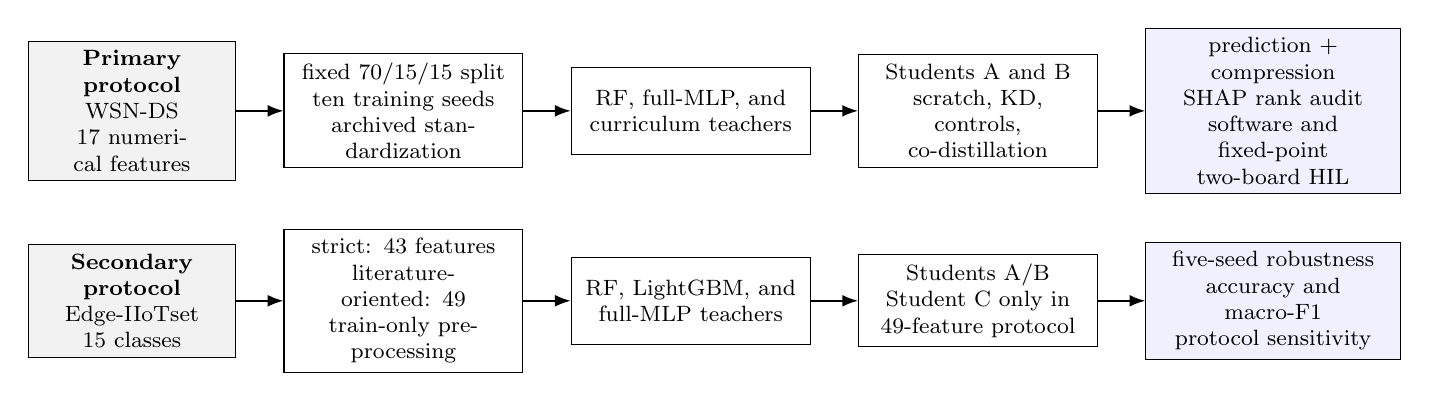
\begin{tikzpicture}[
  source/.style={draw, fill=gray!10, align=center, minimum height=11mm, text width=24mm, font=\footnotesize},
  stage/.style={draw, align=center, minimum height=11mm, text width=28mm, font=\footnotesize},
  outcome/.style={draw, fill=blue!6, align=center, minimum height=11mm, text width=30mm, font=\footnotesize},
  arr/.style={-{Latex[length=2mm]}, semithick},
  node distance=6mm and 6mm
]
\node[source] (wsn) {\textbf{Primary protocol}\\WSN-DS\\17 numerical features};
\node[stage,right=of wsn] (wsnp) {fixed 70/15/15 split\\ten training seeds\\archived standardization};
\node[stage,right=of wsnp] (wsnt) {RF, full-MLP, and\\curriculum teachers};
\node[stage,right=of wsnt] (wsns) {Students A and B\\scratch, KD, controls,\\co-distillation};
\node[outcome,right=of wsns] (wsno) {prediction + compression\\SHAP rank audit\\software and fixed-point\\two-board HIL};

\node[source,below=8mm of wsn] (edge) {\textbf{Secondary protocol}\\Edge-IIoTset\\15 classes};
\node[stage,right=of edge] (edgep) {strict: 43 features\\literature-oriented: 49\\train-only preprocessing};
\node[stage,right=of edgep] (edget) {RF, LightGBM, and\\full-MLP teachers};
\node[stage,right=of edget] (edges) {Students A/B\\Student C only in\\49-feature protocol};
\node[outcome,right=of edges] (edgeo) {five-seed robustness\\accuracy and macro-F1\\protocol sensitivity};

\draw[arr] (wsn)--(wsnp); \draw[arr] (wsnp)--(wsnt); \draw[arr] (wsnt)--(wsns); \draw[arr] (wsns)--(wsno);
\draw[arr] (edge)--(edgep); \draw[arr] (edgep)--(edget); \draw[arr] (edget)--(edges); \draw[arr] (edges)--(edgeo);
\end{tikzpicture}
\caption{Research design. The WSN-DS branch provides the primary compression, explanation, conversion, and HIL evidence. Edge-IIoTset supplies a separately reported robustness study with different data construction.}
\label{fig:pipeline}
\end{figure*}

Table~\ref{tab:protocols} fixes the three experimental contracts before model-level results are introduced. The two Edge-IIoTset protocols are independent experiments rather than alternative preprocessing of one shared split.

\begin{table*}[t]
\caption{Experimental Protocols}
\label{tab:protocols}
\centering
\scriptsize
\setlength{\tabcolsep}{4pt}
\begin{tabular}{>{\raggedright\arraybackslash}p{24mm}rrrr>{\raggedright\arraybackslash}p{31mm}>{\raggedright\arraybackslash}p{62mm}}
\toprule
Protocol / source & Rows & Classes & Features & Seeds & Split & Preprocessing contract \\
\midrule
\dataset{} / WSN-DS CSV & 374,661 & 5 & 17 & 10 & fixed stratified 70/15/15 & Identifier and target removed; \textbf{train-only} \texttt{StandardScaler} fitted on the training partition after the fixed seed-42 split. \\
Edge strict / ML-EdgeIIoT CSV & 157,800 & 15 & 43 & 5 & fixed stratified 70/15/15 & Identifiers, source/payload fields, ports, auxiliary targets, all-missing, and constant columns removed; training-only imputation, categorical encoding, and scaling. \\
Edge literature-oriented / DNN-EdgeIIoT CSV & 2,219,201 & 15 & 49 & 5 & fixed stratified 70/15/15 & Thirteen identifier/source/payload/leakage fields removed while ports are retained; training-only imputation, categorical encoding, and scaling. \\
\bottomrule
\end{tabular}
\end{table*}

\subsection{WSN-DS Data and Split}
The repository copy of \dataset{} contains 374,661 records and 19 columns. Removing the identifier and target leaves 17 numerical features. Class counts are 10,049 Blackhole, 3,312 Flooding, 14,596 Grayhole, 340,066 Normal, and 6,638 TDMA. A fixed stratified 70/15/15 split with random state 42 produces 262,252 training, 56,209 validation, and 56,200 test records. Ten model seeds vary RF randomness and neural initialization while the split remains fixed:
\[
\{42,123,456,789,1001,2024,3141,5678,8192,9999\}.
\]

Primary multi-seed predictive tables use a train-only \texttt{StandardScaler} fitted on the training partition after the fixed seed-42 stratified split (validation/test transform only). An archived pre-split-scaler package is retained for historical comparison and must not be mixed with train-only claims. Deployment evidence uses a separate clean seed-42 RF-KD unit (set\_seed then RF-KD only) with host ONNX/OpenVINO export, fixed-point conversion under a measured 0.03 macro-F1 drop bound, and four full-test MCU replays. Dual identity is explicit: multi-config pipeline seed-42 RF-KD (Student A $0.9203$ class of values near 0.9249) is not the same training unit as deployment-clean seed-42 RF-KD ($\approx0.9485$).

\subsection{Teachers and Compact Students}
The primary tree teacher is an RF with 500 trees and maximum depth 15 \cite{breiman2001random}. For KD, its probabilities are isotonic-calibrated with three-fold cross-validation \cite{guo2017calibration}. The neural teacher is a $17$--$128$--$256$--$128$--$5$ MLP with batch normalization, ReLU, and dropout. It has 69,893 trainable parameters and a 273.02~KB FP32 parameter payload.

Student A is $17$--$32$--$16$--$5$ (1,189 parameters, 1,136 MACs), and Student B is $17$--$64$--$32$--$5$ (3,397 parameters, 3,296 MACs). ReLU follows both hidden layers; the output layer produces five logits. Fig.~\ref{fig:architecture} shows what is transferred, what remains trainable, and which representations are evaluated after training. Both students are independently parameterized fixed-capacity networks.

\begin{figure*}[t]
\centering
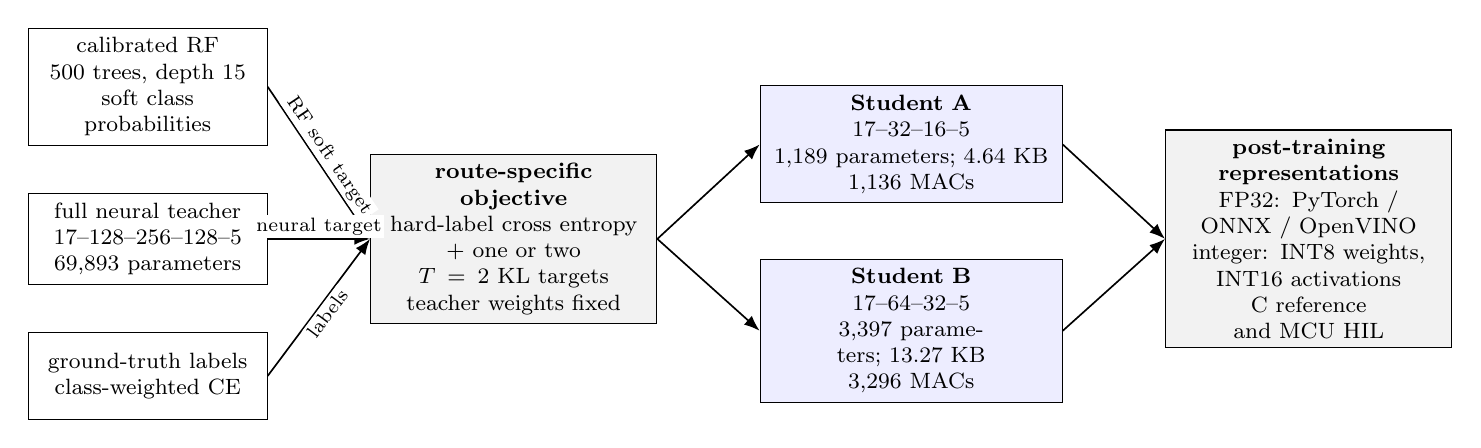
\begin{tikzpicture}[
  block/.style={draw, align=center, minimum height=11mm, text width=28mm, font=\footnotesize},
  objective/.style={draw, fill=gray!10, align=center, minimum height=19mm, text width=34mm, font=\footnotesize},
  student/.style={draw, fill=blue!7, align=center, minimum height=14mm, text width=36mm, font=\footnotesize},
  deploy/.style={draw, fill=gray!10, align=center, minimum height=19mm, text width=34mm, font=\footnotesize},
  arr/.style={-{Latex[length=2mm]}, semithick},
  loss/.style={font=\scriptsize, fill=white, inner sep=1pt},
  node distance=7mm and 9mm
]
\node[block] (rf) {calibrated RF\\500 trees, depth 15\\soft class probabilities};
\node[block,below=6mm of rf] (mlp) {full neural teacher\\17--128--256--128--5\\69,893 parameters};
\node[block,below=6mm of mlp] (hard) {ground-truth labels\\class-weighted CE};

\node[objective,right=13mm of mlp] (obj) {\textbf{route-specific objective}\\hard-label cross entropy\\$+$ one or two $T=2$ KL targets\\teacher weights fixed};

\node[student,right=13mm of obj,yshift=12mm] (a) {\textbf{Student A}\\17--32--16--5\\1,189 parameters; 4.64 KB\\1,136 MACs};
\node[student,below=7mm of a] (b) {\textbf{Student B}\\17--64--32--5\\3,397 parameters; 13.27 KB\\3,296 MACs};

\node[deploy,right=13mm of a,yshift=-12mm] (dep) {\textbf{post-training representations}\\FP32: PyTorch / ONNX / OpenVINO\\integer: INT8 weights, INT16 activations\\C reference and MCU HIL};

\draw[arr] (rf.east) -- node[loss,above,sloped] {RF soft target} (obj.west);
\draw[arr] (mlp.east) -- node[loss,above] {neural target} (obj.west);
\draw[arr] (hard.east) -- node[loss,below,sloped] {labels} (obj.west);
\draw[arr] (obj.east) -- (a.west); \draw[arr] (obj.east) -- (b.west);
\draw[arr] (a.east) -- (dep.west); \draw[arr] (b.east) -- (dep.west);
\end{tikzpicture}
\caption{Compression and deployment structure for WSN-DS. Training routes select one or two teacher targets together with the hard-label term; the student architecture itself is unchanged. Both students are evaluated in FP32/software representations, while the RF-distilled instances are additionally converted to fixed-point C and replayed on both boards. Parameter counts include weights and biases.}
\label{fig:architecture}
\end{figure*}

\subsection{Training Routes}
For target $y$, student logits $z_s$, temperature $T$, and KD weight $\alpha$, define $p_s^{(T)}=\sigma(z_s/T)$. A neural teacher with logits $z_t$ supplies $q_t^{(T)}=\sigma(z_t/T)$. The calibrated RF instead supplies probabilities $r$, clipped below at $10^{-8}$; the implementation uses pseudo-logits $\log r$, so its softened target is
\begin{equation}
q_{\mathrm{RF},i}^{(T)}
=\frac{\exp(\log r_i/T)}{\sum_j\exp(\log r_j/T)}
=\frac{r_i^{1/T}}{\sum_j r_j^{1/T}}.
\label{eq:rf-softening}
\end{equation}
With $q_t^{(T)}$ selected from the neural or RF definition, the single-teacher objective is
\begin{equation}
\mathcal{L}_{\mathrm{KD}}=(1-\alpha)\,\mathcal{L}_{\mathrm{CE}}(z_s,y)
+\alpha T^2 D_{\mathrm{KL}}\!\left(q_t^{(T)}\,\|\,p_s^{(T)}\right).
\label{eq:kd}
\end{equation}
A validation grid over $T\in\{2,3,4,5\}$ and $\alpha\in\{0.5,0.7,0.9\}$ selects $T=2$ and $\alpha=0.5$. Inverse-frequency class weights are used in cross entropy. Standard neural runs use AdamW, learning rate $10^{-3}$, weight decay $10^{-3}$, cosine annealing, batch size 256, 30 epochs, and early-stopping patience eight.

The experiment matrix is summarized in Table~\ref{tab:routes}. Configurations C and F are archival aliases of their nominal-schedule variants and count once in statistical comparisons. The loss curriculum trains a three-epoch probe, orders examples by per-example loss, and exposes 33\%, 66\%, and 100\% of the training set for 3, 3, and 24 nominal epochs. This is not compute matched to 30 full-data epochs because the first stages use subsets and global early stopping can terminate before the final stage. The extended route uses 5, 5, and 30 nominal epochs. Random pacing is the ordering control. The SMOTE route changes the neural teacher's training distribution using synthetic minority oversampling \cite{chawla2002smote}.

\begin{table}[t]
\caption{WSN-DS Experiment Routes}
\label{tab:routes}
\centering
\footnotesize
\begin{tabular}{cll}
\toprule
Code & Model trained & Supervision / schedule \\
\midrule
A & RF-500 & hard labels \\
B & full MLP & hard labels \\
C2 & full MLP & domain curriculum \\
C & full MLP & nominal-schedule loss curriculum (alias) \\
C-ext & full MLP & extended loss curriculum \\
C-fair & full MLP & nominal-schedule loss curriculum \\
D & compact student & hard labels \\
E2 & compact student & full-MLP KD \\
E & compact student & calibrated RF-KD \\
F & compact student & nominal-schedule curriculum-KD (alias) \\
F-ext & compact student & extended curriculum-KD \\
F-fair & compact student & nominal-schedule curriculum-KD \\
G & compact student & random-pacing teacher KD \\
I & compact student & SMOTE-trained MLP KD \\
J & compact student & RF + curriculum co-distillation \\
\bottomrule
\end{tabular}
\end{table}

For co-distillation, let $\mathcal{K}_{\mathrm{RF}}=T^2D_{\mathrm{KL}}(q_{\mathrm{RF}}^{(T)}\|p_s^{(T)})$ and $\mathcal{K}_{\mathrm{CL}}=T^2D_{\mathrm{KL}}(q_{\mathrm{CL}}^{(T)}\|p_s^{(T)})$. Configuration J combines one hard-label term with the two distinct soft-target terms:
\begin{equation}
\mathcal{L}_{J}=0.3\mathcal{L}_{\mathrm{CE}}(z_s,y)
+0.4\mathcal{K}_{\mathrm{RF}}+0.3\mathcal{K}_{\mathrm{CL}}.
\label{eq:co}
\end{equation}
Configuration J uses $T=2$, learning rate $7\times10^{-4}$, 40 epochs, and patience ten. Results are reported with this larger compute budget.

\subsection{Explanation Audit}
TreeExplainer produces RF attributions and DeepExplainer produces Student A attributions \cite{lundberg2017shap}. The preserved audit uses 100 background samples and 500 explained samples. Its student is the final-seed Student A distilled from the nominal-schedule curriculum MLP (the historical F-fair key), not the RF-KD or co-distilled model; this is the only preserved model pair with SHAP evidence. Global importance is the mean absolute SHAP value by feature. Spearman correlation compares the 17 feature ranks. Five repeated subsamples provide descriptive sensitivity through their mean and standard deviation.

\subsection{Software and Fixed-Point Deployment}
The deployment path has four numerical representations:
\begin{enumerate}
  \item PyTorch FP32 and quantization-aware training (QAT) artifacts \cite{paszke2019pytorch};
  \item FP32 and dynamic-INT8 ONNX graphs executed by ONNX Runtime \cite{onnx,onnxruntime};
  \item FP32 ONNX graphs imported by OpenVINO \cite{openvino}; and
  \item generated C with integer StandardScaler preprocessing, INT8 weights, INT32 biases/accumulators, and INT16 layer activations.
\end{enumerate}

Host-runtime measurements use one preserved artifact per route on the recorded Windows 10/Python 3.11.9 environment. Each ONNX Runtime and OpenVINO latency distribution uses 50 warm-up calls followed by 1,000 batch-one and 300 batch-64 timed calls; Table~\ref{tab:runtime} reports the batch-one median and 95th percentile. The archived environment omits the host CPU model, limiting these values to within-machine format comparisons.

The HIL host replays already extracted 17-feature records over USB serial. Firmware performs integer preprocessing and dense inference, then returns status, prediction, and timing. Both RF-KD artifacts originate from the recorded proof run with model seed 9999. The data split uses random state 42, and the exporter records test-vector seed 42; at the full replay count, selection resolves to all ordered test indices 0--56,199. Board timing excludes host serialization and covers on-device preprocessing plus inference. Therefore, HIL establishes fixed-point execution of the tabular detector, not radio capture, packet-to-feature extraction, or end-to-end network throughput.

\subsection{Edge-IIoTset Protocols}
Both Edge-IIoTset studies use seeds $\{42,123,456,789,1001\}$, fixed stratified 70/15/15 splits, and train-only preprocessing. Categorical vocabularies, imputation values, and scaling statistics are learned from the training partition; categorical levels occurring fewer than ten times are grouped and encoded cardinality is capped at 64. Neural training uses the same 30-epoch, batch-256, AdamW schedule as the WSN study. RF teachers use 500 trees, depth 15, and three-fold isotonic calibration. The WSN-selected $T=2$ and $\alpha=0.5$ are transferred without Edge-IIoTset retuning. The literature-oriented protocol additionally evaluates LightGBM with 500 estimators, learning rate 0.05, and 31 leaves.

The \emph{strict} protocol uses the 157,800-row ML-EdgeIIoT file. It removes 16 identifier, source, payload, port, and label-leakage fields, followed by all-missing and constant columns, yielding 43 features and 15 classes. It evaluates Students A and B, whose parameter counts increase to 2,191 and 5,391 because of the larger input and output dimensions.

The \emph{literature-oriented} protocol uses the 2,219,201-row DNN-EdgeIIoT file. It removes 13 identifier/source/payload/leakage fields but retains port fields, yielding 49 features and 15 classes. Students A, B, and C use hidden widths 32--16, 64--32, and 128--64. The protocol name indicates closer alignment with common Edge-IIoT studies; exact cross-paper equivalence still depends on retained fields and preprocessing.

\section{Experimental Evaluation}
\subsection{Metrics and Statistical Scope}
Accuracy is reported for continuity with prior work. Macro-F1 is primary because it weights each class equally. Per-class F1 exposes the Blackhole/Grayhole trade-off obscured by the dominant Normal class. Ten-seed values are mean $\pm$ population standard deviation as stored by the experiment code. Paired, two-sided Wilcoxon signed-rank tests compare seed-level macro-F1 values \cite{wilcoxon1945}. For the ten unique co-distillation comparisons archived across two students, Holm's step-down procedure controls family-wise error; raw and adjusted $p$ values are both reported. These tests remain exploratory because $n=10$ and all seeds share one split.

Latency tables evaluate one preserved artifact per route on its recorded host environment, whereas predictive tables summarize multi-seed training. HIL metrics cover every test record. Model storage is always labeled by basis: serialized pickle, raw FP32 parameter payload, serialized ONNX/PyTorch artifact, fixed-point model-only constants, or framework-linked firmware total.

\subsection{RQ1: Predictive Performance and Compression}
Table~\ref{tab:wsn-main} gives the central ten-seed result. The RF teacher is strongest at $0.97889\pm0.00025$ \mf{}. The 69,893-parameter full MLP reaches $0.92319\pm0.00238$. Student A RF-KD reaches $0.91997\pm0.00312$ in 4.64~KB, 0.00767 above Student A scratch. Student B is stronger by capacity: scratch already reaches 0.93217, RF-KD reaches 0.93281, and co-distillation reaches 0.93353.

\begin{table*}[t]
\caption{Selected WSN-DS Ten-Seed Results under the train-only-scaler protocol (sample std, $n=10$). Neural sizes are raw FP32 parameter payloads; RF size is the recorded mean serialized-pickle size.}
\label{tab:wsn-main}
\centering
\small
\begin{tabular}{llrrrrr}
\toprule
Model & Route & Parameters & Size (KB) & Accuracy & Macro-F1 & $\Delta$F1 vs scratch \\
\midrule
RF teacher & supervised & -- & 85064.54$^\dagger$ & $0.99659\pm0.00006$ & $0.97885\pm0.00025$ & -- \\
Full MLP & supervised & 69,893 & 273.02 & $0.98726\pm0.00030$ & $0.92269\pm0.00190$ & -- \\
Student A & scratch & 1,189 & 4.64 & $0.98436\pm0.00237$ & $0.91090\pm0.00649$ & -- \\
Student A & MLP-KD & 1,189 & 4.64 & $0.98539\pm0.00034$ & $0.91204\pm0.00222$ & +0.00114 \\
Student A & RF-KD & 1,189 & 4.64 & $0.98694\pm0.00101$ & $0.92034\pm0.00618$ & +0.00944 \\
Student A & co-distill & 1,189 & 4.64 & $0.98614\pm0.00040$ & $0.91577\pm0.00259$ & +0.00487 \\
Student B & scratch & 3,397 & 13.27 & $0.98873\pm0.00098$ & $0.93134\pm0.00624$ & -- \\
Student B & MLP-KD & 3,397 & 13.27 & $0.98643\pm0.00072$ & $0.91774\pm0.00434$ & -0.01360 \\
Student B & RF-KD & 3,397 & 13.27 & $0.99019\pm0.00202$ & $0.93917\pm0.01225$ & +0.00783 \\
Student B & co-distill & 3,397 & 13.27 & $0.98890\pm0.00233$ & $0.93225\pm0.01405$ & +0.00091 \\
\bottomrule
\multicolumn{7}{l}{\footnotesize $^\dagger$Serialized RF artifact; its storage representation differs from raw neural parameters.}
\end{tabular}
\end{table*}


\begin{figure}[t]
\centering
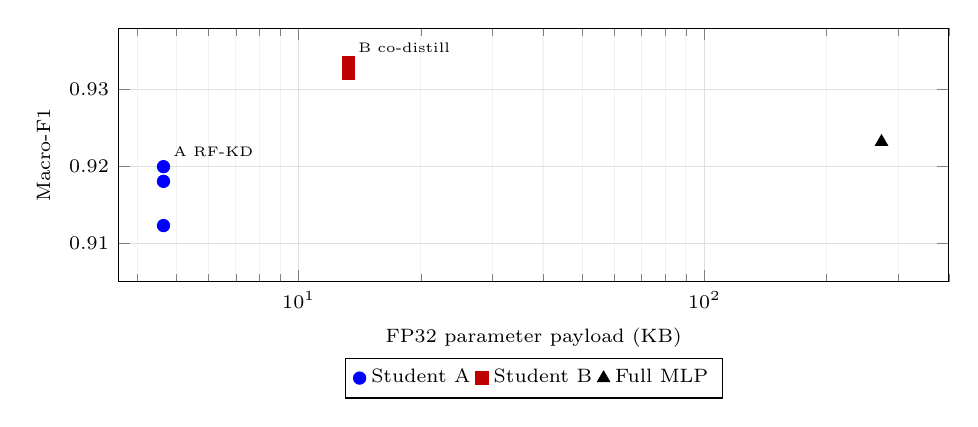
\begin{tikzpicture}
\begin{axis}[
  width=\columnwidth,height=48mm,
  xmode=log,log basis x=10,
  xmin=3.6,xmax=400,ymin=0.905,ymax=0.938,
  xlabel={FP32 parameter payload (KB)},ylabel={Macro-F1},
  grid=both,major grid style={gray!25},minor grid style={gray!10},
  legend style={font=\scriptsize,at={(0.5,-0.30)},anchor=north,legend columns=3},
  tick label style={font=\scriptsize},label style={font=\scriptsize}
]
\addplot[only marks,mark=*,mark size=2.2pt,blue] coordinates {
 (4.64453,0.912303)
 (4.64453,0.919971)
 (4.64453,0.918062) };
\addlegendentry{Student A}
\addplot[only marks,mark=square*,mark size=2.2pt,red!75!black] coordinates {
 (13.26953,0.932169)
 (13.26953,0.932808)
 (13.26953,0.933526) };
\addlegendentry{Student B}
\addplot[only marks,mark=triangle*,mark size=2.5pt,black] coordinates {
 (273.01953,0.923195) };
\addlegendentry{Full MLP}
\node[font=\tiny,anchor=south west] at (axis cs:4.6445,0.919971) {A RF-KD};
\node[font=\tiny,anchor=south west] at (axis cs:13.2695,0.933526) {B co-distill};
\end{axis}
\end{tikzpicture}
\caption{WSN-DS size--performance trade-off. Points are ten-seed means; all configurations at a student capacity share the same FP32 parameter size.}
\label{fig:wsn-tradeoff}
\end{figure}


Table~\ref{tab:per-class} shows why aggregate accuracy is insufficient. Student A RF-KD is stronger than Student A co-distillation on Blackhole and Grayhole. Student B co-distillation has the best Student B Blackhole F1 (0.878) but RF-KD has stronger Grayhole F1 (0.902 versus 0.891). The Normal class remains near 0.998 for all selected students.

\begin{table}[t]
\caption{Selected WSN-DS Mean Per-Class F1}
\label{tab:per-class}
\centering
\scriptsize
\setlength{\tabcolsep}{3pt}
\begin{tabular}{lrrrrrr}
\toprule
Model & BH & Flood & Gray & Normal & TDMA & Macro \\
\midrule
\primitiveinput generated/wsn_selected_per_class_rows.tex 
\bottomrule
\end{tabular}
\end{table}

\subsection{Compression Accounting}
The commonly quoted RF-to-student ratios compare an 85,064.54~KB serialized RF pickle with raw FP32 neural parameters. Under that mixed but explicit basis, Student A and B are 18,315$\times$ and 6,411$\times$ smaller. The same-basis neural comparison is cleaner: relative to the full MLP's FP32 parameter payload, Students A and B are 58.8$\times$ and 20.6$\times$ smaller. ONNX serialization produces 5.44 and 14.07~KB artifacts. Fixed-point model constants require 1,348 and 3,700 bytes, excluding code, preprocessing constants, buffers, protocol, and board framework.

\begin{table}[t]
\caption{Storage Measurements and Their Meaning}
\label{tab:storage}
\centering
\footnotesize
\begin{tabular}{lrl}
\toprule
Artifact & Size & Measurement basis \\
\midrule
RF teacher & 85,064.54 KB & serialized pickle \\
Full MLP & 273.02 KB & raw FP32 parameters \\
Student A & 4.64 KB & raw FP32 parameters \\
Student B & 13.27 KB & raw FP32 parameters \\
Student A ONNX & 5.44 KB & serialized FP32 graph \\
Student B ONNX & 14.07 KB & serialized FP32 graph \\
Student A fixed core & 1,348 B & weights + biases only \\
Student B fixed core & 3,700 B & weights + biases only \\
\bottomrule
\end{tabular}
\end{table}

\subsection{RQ2: Effects of Distillation and Curriculum}
The complete route matrices appear in Appendix~\ref{app:results}. Three conclusions follow.

First, RF-KD is the most reliable Student A route. Its mean \mf{} is 0.91997, compared with 0.91635 for MLP-KD and 0.91291 for nominal-schedule curriculum-KD. Second, Student B gains little from KD because scratch training is already strong. MLP-KD lowers Student B \mf{} by 0.00462, whereas RF-KD and co-distillation improve it by only 0.00064 and 0.00136. Third, longer curriculum training is unstable: the extended full MLP has $0.86726\pm0.15482$ \mf{}, and extended curriculum-KD has standard deviations near 0.025 for both students. The additional nominal epochs increase variance without a reliable gain.

Table~\ref{tab:wilcoxon} reports the paired co-distillation comparisons. After Holm adjustment, Student A co-distillation is better than nominal-schedule curriculum-KD (mean difference 0.0051, $p_{\mathrm{Holm}}=0.0352$) but worse than the full MLP (mean difference $-0.0051$, $p_{\mathrm{Holm}}=0.0195$). Its differences from Student A scratch, RF-KD, and MLP-KD are not significant. No Student B comparison survives adjustment: in particular, the 0.0014 mean gain over scratch and 0.0007 gain over RF-KD are unsupported. The tests therefore reject universal co-distillation superiority and show that the apparent Student B advantages in raw $p$ values are not robust to family-wise correction.

\begin{table}[t]
\caption{Co-Distillation Paired Wilcoxon Tests on WSN-DS Macro-F1. Holm adjustment covers the ten unique comparisons shown.}
\label{tab:wilcoxon}
\centering
\scriptsize
\setlength{\tabcolsep}{2.5pt}
\begin{tabular}{clrrrr}
\toprule
Student & Comparator & Mean diff. & $W$ & $p_{\mathrm{raw}}$ & $p_{\mathrm{Holm}}$ \\
\midrule
\primitiveinput generated/wsn_codistill_wilcoxon_rows.tex 
\bottomrule
\end{tabular}
\end{table}

\subsection{RQ3: Explanation Fidelity}
The audited Student A curriculum-KD model and RF reference have global rank correlation $\rho=\ShapRho$ with $p=\ShapP$. Across five repeated subsamples, mean $\rho$ is \ShapRepeatMean{} with standard deviation \ShapRepeatStd{}. Per-class correlations are 0.211 (Blackhole), 0.409 (Flooding), $-0.015$ (Grayhole), $-0.081$ (Normal), and $-0.150$ (TDMA); none is significant in the preserved output. Because this student was distilled from the curriculum MLP rather than the RF, the comparison measures cross-model alignment and cannot establish attribution transfer from the actual distillation teacher.

The mismatch extends across the ranking. The student's five leading features are \texttt{Is\_CH}, \texttt{Time}, \texttt{who CH}, \texttt{dist\_CH\_To\_BS}, and \texttt{Data\_Sent\_To\_BS}. The RF's five are \texttt{ADV\_S}, \texttt{Is\_CH}, \texttt{Data\_Sent\_To\_BS}, \texttt{DATA\_S}, and \texttt{Expaned Energy}. Table~\ref{tab:shap-ranks} provides all 17 ranks. The result answers RQ3 negatively for this model pair; Student B, RF-KD, and co-distillation lack corresponding attribution audits.

\begin{table}[t]
\caption{Global SHAP Feature Ranks for the Audited Pair}
\label{tab:shap-ranks}
\centering
\scriptsize
\begin{tabular}{lrrr}
\toprule
Feature & RF rank & Student rank & $\Delta$rank \\
\midrule
\primitiveinput generated/shap_rank_rows.tex 
\bottomrule
\end{tabular}
\end{table}

\subsection{RQ4: Software Runtime and Quantization}
\subsubsection{PyTorch QAT}
QAT was evaluated for D, E, and J at one proof seed (9999) on the recorded Windows/PyTorch environment. Table~\ref{tab:qat} shows that all six QAT artifacts lose \mf{} relative to their corresponding FP32 artifacts. The smallest drop is 0.00414 for Student A co-distillation; the largest is 0.02336 for Student B RF-KD. These runs establish convertibility with measured, model-dependent loss.

\begin{table}[t]
\caption{Single-Artifact PyTorch QAT Results}
\label{tab:qat}
\centering
\scriptsize
\begin{tabular}{lrrr}
\toprule
Model & Accuracy & Macro-F1 & $\Delta$ vs FP32 \\
\midrule
\primitiveinput generated/qat_all_rows.tex 
\bottomrule
\end{tabular}
\end{table}

\subsubsection{ONNX Runtime and OpenVINO}
FP32 ONNX batch-one median latency is 0.0267--0.0289~ms for the six compact artifacts. OpenVINO produces identical predictions to ONNX in every evaluated pair, but median latency is about 0.129--0.132~ms in this environment. Dynamic INT8 ONNX reduces Student B graph size from 14.07 to 7.37~KB, but lowers \mf{} and has a slower batch-one median (approximately 0.039--0.040~ms) than ONNX FP32. Table~\ref{tab:runtime} reports all 18 runtime rows; on this host, neither lower precision nor OpenVINO improves latency.

\begin{table*}[t]
\caption{Single-Artifact ONNX/OpenVINO Runtime Results}
\label{tab:runtime}
\centering
\scriptsize
\setlength{\tabcolsep}{4pt}
\begin{tabular}{llrrrrrr}
\toprule
Model & Runtime & Accuracy & Macro-F1 & Size KB & p50 ms & p95 ms & Agreement \\
\midrule
\primitiveinput generated/runtime_all_rows.tex 
\bottomrule
\end{tabular}
\end{table*}

\subsubsection{Fixed-Point HIL Fidelity}
Table~\ref{tab:hil} is the strongest executable evidence. All four model--board pairs completed 56,200 vectors with no missing, duplicate, unexpected, or non-OK responses. MCU predictions agree 100\% with generated fixed-point references. Agreement with FP32 is 0.9950 for Student A and 0.9939 for Student B, so remaining differences arise from fixed-point conversion rather than serial transport or board-specific execution.

\begin{table*}[t]
\caption{Full-Test-Set Fixed-Point HIL Results}
\label{tab:hil}
\centering
\small
\begin{tabular}{llrrrrrr}
\toprule
Model & Board & Vectors & Macro-F1 & MCU/fixed & MCU/FP32 & Mean total $\mu$s & p99 $\mu$s \\
\midrule
\primitiveinput generated/hil_fidelity_rows.tex 
\bottomrule
\end{tabular}
\end{table*}


\begin{figure}[t]
\centering
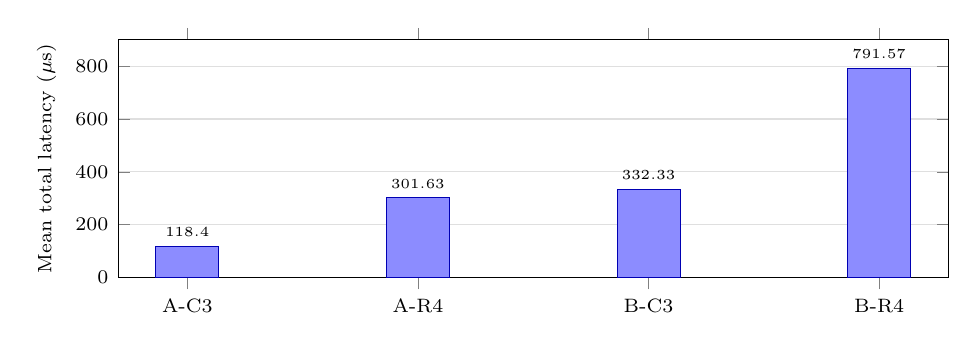
\begin{tikzpicture}
\begin{axis}[
  width=\columnwidth,height=46mm,ybar,bar width=8mm,
  symbolic x coords={A-C3,A-R4,B-C3,B-R4},xtick=data,
  ymin=0,ymax=900,ylabel={Mean total latency ($\mu$s)},
  nodes near coords,nodes near coords style={font=\tiny},
  tick label style={font=\scriptsize},label style={font=\scriptsize},
  ymajorgrids=true,major grid style={gray!25}
]
\addplot[fill=blue!45,draw=blue!70!black] coordinates {
 (A-C3,118.40) (A-R4,301.63)
 (B-C3,332.33) (B-R4,791.57) };
\end{axis}
\end{tikzpicture}
\caption{Measured fixed-point preprocessing-plus-inference latency over all 56,200 records. C3 denotes ESP32-C3 and R4 denotes Arduino UNO R4 WiFi.}
\label{fig:hil-latency}
\end{figure}


Student A is faster because it performs 1,136 rather than 3,296 MACs. Table~\ref{tab:cycles} normalizes timing. ESP32-C3 requires approximately 15.8 cycles/MAC for either model, while R4 requires 11.2--11.8. The compute-only processing ceilings range from 1,263 to 8,446 vectors/s. These are reciprocals of on-device preprocessing-plus-inference time, not serial or radio throughput.

\begin{table}[t]
\caption{HIL Compute Normalization}
\label{tab:cycles}
\centering
\scriptsize
\setlength{\tabcolsep}{3pt}
\begin{tabular}{llrrrrr}
\toprule
Model & Board & MACs & Inf. $\mu$s & Cycles & cyc/MAC & vec/s \\
\midrule
\primitiveinput generated/hil_cycles_rows.tex 
\bottomrule
\end{tabular}
\end{table}

Fixed-point drift affects 281 Student A records (0.500\%) and 343 Student B records (0.610\%). Student A drift is concentrated in Blackhole (107) and Grayhole (150), with 23 Normal and one TDMA record. Student B drift contains 261 Blackhole, 65 Grayhole, 16 Normal, and one TDMA record. Neither model changes a Flooding prediction relative to FP32. Thus a single agreement percentage hides class-specific numerical sensitivity.

\subsubsection{Train-Only Scaler Deployment Confirmation}
To address the pre-split scaling limitation for executable claims, RF-KD Students A and B were retrained at seed 42 with a train-fitted \texttt{StandardScaler} on the same archived split indices. Host ONNX Runtime evaluation of the train-only FP32 graphs matches PyTorch on every test record (agreement 1.0); OpenVINO CPU execution of the same ONNX graphs also agrees exactly with PyTorch and ONNX Runtime (agreement 1.0) with batch-one median latency about 0.110--0.114~ms on the evaluation host. Dynamic INT8 ONNX reduces macro-F1 (Student A $0.9485\rightarrow0.8938$, Student B $0.9449\rightarrow0.9066$) and is retained only as a software-size probe. Direct post-training fixed-point conversion of the train-only FP32 weights was selected for MCU export after a QAT refine probe lowered absolute Student A macro-F1. On ESP32-C3 and Arduino UNO R4 WiFi, all four train-only model--board pairs completed 56,200 serial replays with 100\% MCU-to-fixed-reference agreement and all-OK status; MCU-to-FP32 agreement is 0.9919 (A) and 0.9905 (B), matching the export conversion gap. Board mean total latency is 116.5~$\mu$s (ESP32-C3 Student A), 320.3~$\mu$s (ESP32-C3 Student B), 301.5~$\mu$s (R4 Student A), and 791.4~$\mu$s (R4 Student B). Fixed MCU macro-F1 is 0.9244 (A) and 0.9180 (B). Arduino CLI recompiles on the HIL host record flash footprints of 281.8--284.1~KB (ESP32-C3) and 56.4--58.7~KB (R4) with ID-bound binaries; post-flash 10-row smokes on all four pairs returned 10/10 OK. Artifacts live under copy-suffixed paths so archived tables remain unaltered.

A separate five-seed exact-feature-group sensitivity package (seeds $\{42,123,456,789,1001\}$, train-only scaler, partitions disjoint on identical feature vectors) yields RF-KD mean \mf{} $0.9141\pm0.0069$ (Student A) and $0.9281\pm0.0074$ (Student B). Mean paired KD-minus-scratch \mf{} deltas are near zero ($+0.0002$ for A, $-0.0017$ for B). That package is a descriptive leakage-control sensitivity analysis, not a matched causal ablation of the archived random-row route and not a significance claim.

\begin{table}[t]
\caption{Fixed-Point Model Core and Prediction Drift}
\label{tab:drift}
\centering
\scriptsize
\begin{tabular}{llrrrr}
\toprule
Model & Architecture & MACs & Param B & Drift & Drift \% \\
\midrule
\primitiveinput generated/hil_model_drift_rows.tex 
\bottomrule
\end{tabular}
\end{table}

\subsubsection{Framework-Linked Compile Footprint}
Arduino compile totals include board support and serial replay code. To isolate the incremental payload, Table~\ref{tab:compile} subtracts a serial-only baseline compiled for the same board environment. Program deltas are 4,248--7,036 bytes and global-variable deltas are 388--392 bytes. These deltas are more informative for model integration than presenting the 278--281~KB ESP32 framework total as model size.

\begin{table}[t]
\caption{Board Compilation Totals and Baseline Deltas}
\label{tab:compile}
\centering
\scriptsize
\setlength{\tabcolsep}{2.2pt}
\begin{tabular}{llrrrr}
\toprule
Model & Board & Prog. B & Glob. B & $\Delta$prog. & $\Delta$glob. \\
\midrule
\primitiveinput generated/hil_compile_rows.tex 
\bottomrule
\end{tabular}
\end{table}

\subsubsection{MSP430F1611 Memory Feasibility}
The Student A preprocessing and inference core was cross-compiled for MSP430F1611 using MSP430-GCC 9.3.1.11 with \texttt{-Os}. The linked smoke firmware reports 2,842 bytes of text-class storage, zero data bytes, six BSS/heap bytes, and a conservative project-function stack estimate of about 248 bytes during prediction. The inference object contributes 494~B \texttt{.text} and 1,348~B \texttt{.rodata}; preprocessing contributes 412~B \texttt{.text} and 136~B \texttt{.rodata}. This supports memory feasibility against the nominal 48~KB flash and 10~KB RAM of the target class. Wider arithmetic invokes MSP430 helper routines, so static size alone cannot predict cycle latency. Physical TelosB execution remains future work.

\subsection{RQ5: Edge-IIoTset Robustness}
Table~\ref{tab:edge-main} summarizes the two protocols. Under strict feature removal, the RF teacher reaches 0.8729 \mf{}, whereas the best compact model is Student B RF-KD at 0.7111. Co-distillation is nearly tied at 0.7100. Under the literature-oriented protocol, RF reaches 0.8892, LightGBM reaches 0.8861, and Student C RF-KD reaches 0.8244 in 61.06~KB. Student C scratch is only 0.00047 lower, and Student B LightGBM-KD is 0.00302 above Student B scratch. KD benefits are therefore small and architecture-dependent.

\begin{table*}[t]
\caption{Selected Edge-IIoTset Five-Seed Results}
\label{tab:edge-main}
\centering
\small
\begin{tabular}{lllrrrr}
\toprule
Protocol & Model & Route & Parameters & Size KB & Accuracy & Macro-F1 \\
\midrule
Strict (43 feat.) & RF & supervised & -- & 109,879.57 & $0.8833\pm0.0002$ & $0.8729\pm0.0002$ \\
Strict (43 feat.) & Student A & scratch & 2,191 & 8.56 & $0.7001\pm0.0191$ & $0.6646\pm0.0200$ \\
Strict (43 feat.) & Student A & co-distill & 2,191 & 8.56 & $0.7243\pm0.0057$ & $0.7010\pm0.0065$ \\
Strict (43 feat.) & Student B & scratch & 5,391 & 21.06 & $0.7236\pm0.0011$ & $0.6878\pm0.0018$ \\
Strict (43 feat.) & Student B & RF-KD & 5,391 & 21.06 & $0.7309\pm0.0031$ & $\mathbf{0.7111}\pm0.0025$ \\
\midrule
Literature (49 feat.) & RF & supervised & -- & 101,114.94 & $0.9825\pm0.0003$ & $0.8892\pm0.0011$ \\
Literature (49 feat.) & LightGBM & supervised & -- & 15,224.05 & $0.9867\pm0.0001$ & $0.8861\pm0.0003$ \\
Literature (49 feat.) & Student A & LightGBM-KD & 2,383 & 9.31 & $0.9661\pm0.0013$ & $0.8143\pm0.0039$ \\
Literature (49 feat.) & Student B & LightGBM-KD & 5,775 & 22.56 & $0.9680\pm0.0002$ & $0.8220\pm0.0010$ \\
Literature (49 feat.) & Student C & scratch & 15,631 & 61.06 & $0.9687\pm0.0001$ & $0.8239\pm0.0003$ \\
Literature (49 feat.) & Student C & RF-KD & 15,631 & 61.06 & $0.9685\pm0.0002$ & $\mathbf{0.8244}\pm0.0009$ \\
\bottomrule
\end{tabular}
\end{table*}


\begin{figure}[t]
\centering
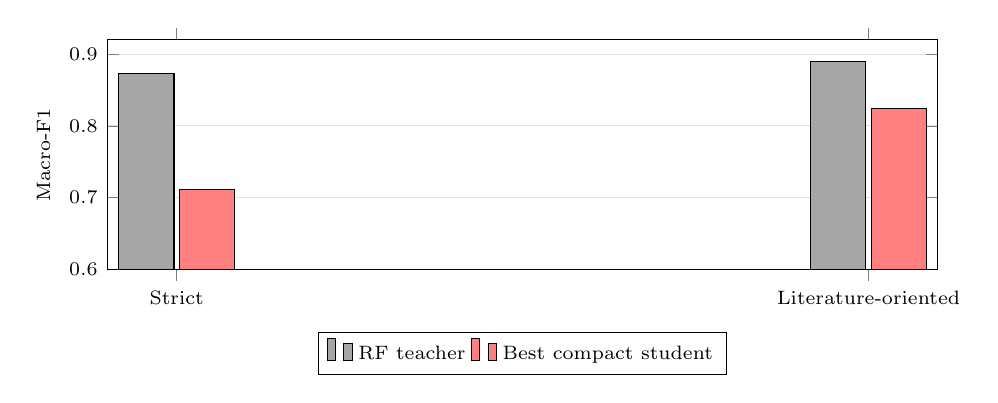
\begin{tikzpicture}
\begin{axis}[
  width=\columnwidth,height=45mm,ybar,bar width=7mm,
  symbolic x coords={Strict,Literature-oriented},xtick=data,
  ymin=0.60,ymax=0.92,ylabel={Macro-F1},
  legend style={font=\scriptsize,at={(0.5,-0.27)},anchor=north,legend columns=2},
  tick label style={font=\scriptsize},label style={font=\scriptsize},
  ymajorgrids=true,major grid style={gray!25}
]
\addplot[fill=black!35] coordinates {(Strict,0.872913) (Literature-oriented,0.889193)};
\addplot[fill=red!50] coordinates {(Strict,0.711114) (Literature-oriented,0.824382)};
\legend{RF teacher,Best compact student}
\end{axis}
\end{tikzpicture}
\caption{Protocol sensitivity on Edge-IIoTset. The protocols use different source files and retained features, so the gap is not attributed to training alone.}
\label{fig:edge-protocol}
\end{figure}


The 0.1133 \mf{} difference between the best compact strict and literature-oriented results arises alongside changes in source file, retained features, and input distribution. This protocol sensitivity is itself a robustness finding and cautions against comparing Edge-IIoTset scores across different identifier, payload-field, or port-retention policies.

\section{Comparison with Prior Work}
Tables~\ref{tab:literature} and \ref{tab:literature-cross} separate direct \dataset{} comparisons from cross-dataset compression and deployment studies. Metric labels retain each source's terminology, including unspecified F1 averaging. \method{} trails the strongest \dataset{} ensembles in raw performance. Its differentiating evidence is the combination of KB-scale dense students, full-test-set fixed-point execution, and a quantitative RF-reference/student explanation audit.

\begin{table*}[t]
\caption{Positioning Against Closely Related Work. Values use each paper's protocol and are not assumed directly comparable.}
\label{tab:literature}
\centering
\scriptsize
\setlength{\tabcolsep}{4pt}
\begin{tabular}{>{\raggedright\arraybackslash}p{28mm}>{\raggedright\arraybackslash}p{22mm}>{\raggedright\arraybackslash}p{31mm}>{\raggedright\arraybackslash}p{29mm}>{\raggedright\arraybackslash}p{47mm}}
\toprule
Work & Dataset / task & Reported predictive result & Reported deployment evidence & Relation to CuKD-XAI \\
\midrule
Almomani \emph{et al.} \cite{almomani2016wsnds} & WSN-DS, 5 class & dataset baselines & none & Defines the primary task and features. \\
Alqahtani \emph{et al.} \cite{alqahtani2019gxgboost} & WSN-DS, 5 class, 10-fold & detection rate 92.9--99.9\% by class & 1.905 s classification time for their test set & Strong class-sensitive tree baseline; no model-size or device result. \\
Salmi and Oughdir \cite{salmi2022cnnlstm} & WSN-DS, 5 class & 0.944 accuracy; 0.959 precision; 0.922 recall & absolute size/latency not reported & Earlier CNN--LSTM baseline under a different split/training protocol. \\
MLSTL-WSN \cite{talukder2024mlstl} & WSN-DS, multiclass & 99.92\% accuracy & 46\% modeling-time reduction; absolute artifact size not reported & Stronger accuracy; uses SHAP for selection, not cross-model explanation agreement. \\
Talukder \emph{et al.} \cite{talukder2025hybrid} & WSN-DS, multiclass & 99.94\% accuracy and reported F1 & absolute size/latency not reported & Stronger predictive result using balancing, PCA, and RF. \\
Birahim \emph{et al.} \cite{birahim2025pso} & WSN-DS, multiclass & 99.73\% accuracy; 99.72\% reported F1 & absolute size/latency not reported & Stronger ensemble accuracy and SHAP/LIME; no compressed neural firmware path. \\
Nguyen \emph{et al.} \cite{nguyen2024gswo} & WSN-DS, multiclass & 99.62\% accuracy in the primary report & absolute size/latency not reported & Optimized CatBoost is predictively stronger; model-core deployment is not evaluated. \\
Xiao and Duan \cite{xiao2025ensemble} & WSN-DS, multiclass & 95.62\% accuracy; 96.07\% reported F1 & approximately 125 MB memory and 175 min training in the local paper & CuKD-XAI accuracy is higher and artifacts are much smaller; F1 averaging differs/unspecified. \\
Alfarra and AbuSamra \cite{alfarra2025energy} & WSN-DS hybrid 4-class gateway path & 98\% accuracy; 0.93 macro-F1 & pruned INT8 CNN--LSTM, 42 ms and 28 mJ/window, lifetime simulation & Closest energy-aware comparator; their energy evidence is stronger, ours covers five-class MCU model-core execution. \\
\method{} (archived protocol) & WSN-DS, 5 class, fixed split & Student A: $0.98688$ accuracy, $0.91997$ macro-F1; Student B: $0.98913$, $0.93353$ & 4.64/13.27 KB FP32 parameters; four full-test HIL replays & Lower predictive ceiling; substantially stronger numerical and execution trace, subject to the disclosed scaling limitation. \\
\bottomrule
\end{tabular}
\end{table*}

\begin{table*}[t]
\caption{Cross-Dataset Compression, Explainability, and Deployment Context. Reported values retain each source's task and measurement boundary.}
\label{tab:literature-cross}
\centering
\scriptsize
\setlength{\tabcolsep}{4pt}
\begin{tabular}{>{\raggedright\arraybackslash}p{28mm}>{\raggedright\arraybackslash}p{24mm}>{\raggedright\arraybackslash}p{35mm}>{\raggedright\arraybackslash}p{36mm}>{\raggedright\arraybackslash}p{34mm}}
\toprule
Work & Dataset / task & Reported predictive result & Reported efficiency / deployment evidence & Relevance and boundary \\
\midrule
Benaddi \emph{et al.} \cite{benaddi2025lightweight} & TON\_IoT, 9 class & 0.9968 accuracy; 0.9863 macro-F1 & 3,042 parameters, 22.29 KB, 1.29 ms & Closest compact KD+SHAP design; different dataset and no fixed-point HIL. \\
Wisanwanichthan and Thammawichai \cite{wisanwanichthan2025kd} & five IoT/UAV IDS datasets & up to 6.12\% improvement reported with KD & 92--95\% parameter reduction; 7--11\% faster inference & Broad KD evidence; reductions are relative and dataset-specific. \\
Javed \emph{et al.} \cite{javed2024thermostat} & smart-thermostat IDS & device-specific binary/multiclass results & quantized CatBoost/XGBoost executed on ESP32 & Stronger application-integrated device study; different traffic and features. \\
Diab \emph{et al.} \cite{diab2025hardware} & Edge-IIoTset, 15 class & 95.25\% LightGBM; 96.73\% HW-NAS CNN accuracy & 74.93 KB/1.20K ops; 190.34 KB/838.89K FLOPs & Hardware-aware baseline; retained features and F1 definition differ. \\
Gao \emph{et al.} \cite{gao2026lightweight} & DNN-EdgeIIoT, 15 class & 93.79--94.24\% accuracy & 16.25--25.37 KB TCN & Compact Edge-IIoT comparison; no common preprocessing contract. \\
Hasan \emph{et al.} \cite{hasan2025autoencoder} & Edge-IIoTset, binary/15 class & 99.94\% accuracy and reported F1 & 0.185/0.187 ms binary/multiclass inference on Jetson Nano & Physical edge timing; tree pipeline and protocol differ. \\
Badhan \cite{badhan2026neurosymbolic} & Edge-IIoTset & 94.3\% accuracy; 93.5\% macro-F1 & 37\% memory and 54\% latency reduction vs. stated baselines & KD plus symbolic explanations; reductions are relative, not artifact bytes. \\
Adjewa \emph{et al.} \cite{adjewa2026seed} & transformer-assisted IoT IDS & 99.9\% accuracy & 137 KB end-device network; under 70 ms on CPU & Offloaded-embedding architecture; system boundary differs from local tabular inference. \\
Nugraha \emph{et al.} \cite{nugraha2025versatile} & three IDS traces & at least 99\% reported F1 & LIME time reduced from 36 to 4.9 s after feature reduction & Stronger cross-explainer/runtime study; no compact-model comparison or MCU result. \\
\bottomrule
\end{tabular}
\end{table*}

Two comparisons should not be collapsed. First, the 18,315$\times$ RF-to-Student-A ratio is larger than ratios reported by many neural compression papers partly because a Python RF pickle and raw neural weights have different serialization overhead. Second, sub-millisecond HIL model-core timing cannot be compared with a gateway window that includes a different feature window and system boundary. The table is therefore positioning evidence, not a universal leaderboard.

\section{Discussion}
\subsection{Answers to the Research Questions}
\textbf{RQ1:} Useful minority-sensitive performance survives large compression, but the RF gap remains. Student A RF-KD loses 0.0589 \mf{} relative to RF while reducing the stated artifact basis from 85,064.54~KB to 4.64~KB. Student B co-distillation loses 0.0454 and uses 13.27~KB. Relative to the full MLP on the same FP32 parameter basis, Student B is 20.6$\times$ smaller and 0.0103 higher in mean \mf{}.

\textbf{RQ2:} Teacher choice matters more than curriculum complexity. RF-KD is best by mean \mf{} for Student A; Student B scratch, RF-KD, and co-distillation are effectively close. Curriculum-only teachers do not improve either capacity, and extended curricula are unstable. After Holm correction, Student A co-distillation improves on nominal-schedule curriculum-KD but remains below the full MLP, while no Student B comparison is significant.

\textbf{RQ3:} The audited student does not align with the RF reference's global SHAP ranking. Predictive utility and cross-model explanation similarity must therefore be reported independently. This finding is specific to one final-seed Student A curriculum-KD/RF-reference pair and motivates a matched-teacher, multi-seed explanation study.

\textbf{RQ4:} The selected RF-KD students are executable with exact generated-integer-reference fidelity on both boards. Quantization introduces 0.50--0.61\% prediction drift relative to FP32, concentrated in Blackhole and Grayhole. Dynamic INT8 ONNX and QAT both introduce \mf{} loss, and dynamic INT8 is slower than FP32 ONNX on the recorded host.

\textbf{RQ5:} Compact students transfer to Edge-IIoTset, but protocol and capacity dominate the result. The best compact \mf{} ranges from 0.7111 to 0.8244 across the two protocols, and the modest KD gains indicate dataset-specific behavior.

\subsection{What the Hardware Results Establish}
The HIL experiment is stronger than a desktop C self-test because the same integer kernels execute on two different MCU architectures and reproduce 56,200 generated references exactly. Compile deltas and fixed-point constants also show that the model core is small relative to board frameworks. The MSP430 cross-compile extends memory feasibility to a WSN-mote-class target. The train-only seed-42 four-pair matrix repeats that full-test fidelity under train-fitted scaling, confirming that exact MCU-to-fixed agreement is not an artifact of the archived pre-split scaler alone.

The experiment still begins with extracted tabular records. It does not implement a LEACH monitor, derive \dataset{} features from packets, run TinyOS/Contiki/RIOT, measure radio traffic, or quantify energy. Those are system-integration questions beyond the current evidence. Describing this boundary precisely makes the HIL result useful rather than weak: it isolates and validates the detector's numerical core.

\subsection{Deployment Choice}
Student A RF-KD is the preferred minimum-footprint configuration. It is the fastest board model and the most reliable Student A route. Student B RF-KD is the conservative higher-capacity deployment choice because it nearly matches Student B co-distillation while using a simpler training target and producing the existing fixed-point artifact. Student B co-distillation is the best mean ten-seed Student B result, but its higher variance and nonsignificant gain over scratch/RF-KD do not justify calling it uniformly superior.

\section{Threats to Validity}
\subsection{Internal Validity}
Primary multi-seed \dataset{} tables now use train-only scaling; residual threats are split sharing (ten seeds, one fixed split), dual training identity (multi-config pipeline vs deployment-clean RF-KD), and curriculum-ext instability (seed 5678 macro-F1 collapse to $\approx0.41$; extended teacher mean $0.867\pm0.162$). Feature-group-disjoint partitions are a descriptive leakage-control sensitivity analysis, not a matched causal ablation. Fixed-point export uses a measured 0.03 macro-F1 drop bound (policy B), not a 0.01-strict gate. Edge literature-comparable random-row splits expose substantial exact-feature cross-partition groups ($\approx17\%$ of test rows); group-aware results must be cited when making leakage-safe Edge claims.

The ten seeds share one train/validation/test split, so variability estimates stochastic training rather than split uncertainty. KD hyperparameters were selected on the seed-42 validation route and then reused. The co-distillation and extended curriculum routes also use larger epoch budgets. The paired Wilcoxon family is Holm-adjusted, but inference remains low-powered at ten paired seeds and does not capture split uncertainty.

\subsection{Construct Validity}
Macro-F1 is primary but omits attack costs. Serialized RF size, FP32 parameter size, fixed-point constants, and linked firmware measure different constructs. Ratios across these bases are explicitly labeled. Reported compute ceilings exclude serial/radio transfer. Runtime benchmarks come from one host and support within-host comparisons.

SHAP agreement compares TreeExplainer and DeepExplainer outputs, so low agreement can reflect both model behavior and explainer/model-class differences. Only one final-seed Student A curriculum-KD pair was audited. Five repeated subsamples provide descriptive sensitivity summaries.

\subsection{External Validity}
\dataset{} is simulated and heavily dominated by Normal traffic. Edge-IIoTset broadens the attack taxonomy but also shows that results depend strongly on source file and retained fields. Live WSN efficacy remains outside both dataset studies. Development-board HIL validates the integer model core, while MSP430 evidence is cross-compile-only. Energy, radio integration, online feature extraction, temporal drift, and adversarial robustness remain unevaluated.

\section{Reproducibility and Artifact Traceability}
All numerical table fragments are regenerated from versioned CSV, JSON, and compiler-log evidence. The generator verifies expected result counts, complete HIL sequences, and compiler totals, then records SHA-256 digests for every consumed source. Complete WSN route matrices, host-runtime rows, board replays, Edge-IIoT rankings, and build logs accompany the manuscript, together with a claim-to-artifact ledger. The implementation uses scikit-learn \cite{pedregosa2011scikit} and PyTorch \cite{paszke2019pytorch}; venue-specific code and data availability text will identify the archival release used for review.

\section{Conclusion}
\method{} shows that WSN intrusion-detector compression must be evaluated across prediction, explanation, numerical conversion, and execution. Under the train-only-scaler \dataset{} protocol, 1,189- and 3,397-parameter RF-KD students retain $0.9203\pm0.0062$ and $0.9392\pm0.0123$ mean \mf{} in 4.64 and 13.27~KB of FP32 parameters (KD$-$scratch $+0.0094$ / $+0.0078$). That KD margin is not guaranteed under feature-group-disjoint splits. Deployment RF-KD global SHAP ranks do not match the RF teacher ($\rho\approx0.238/0.225$, non-significant). Fixed-point conversion incurs class-concentrated drift ($\approx0.024$--$0.027$ macro-F1) even though MCU execution exactly matches the integer reference (agree$=1.0$ on four full-test pairs). Train-only co-distillation reaches $0.9158\pm0.0026$ (A) and $0.9323\pm0.0141$ (B) and must be compared to RF-KD rather than asserted superior a priori. Edge-IIoTset results remain protocol-dependent; literature random-row leakage must be disclosed or removed via group-aware splits. Live feature extraction and energy evaluation remain necessary before complete-system deployment claims.

\appendices
\section{Complete Result Matrices}
\label{app:results}
Tables~\ref{tab:wsn-a-all}--\ref{tab:edge-comparable-all} contain every stored WSN-DS student route and every unique Edge-IIoTset configuration. The WSN-DS C and F aliases duplicate their historical nominal-schedule variants and are retained for traceability; shared Edge-IIoTset teacher rows duplicated under each student-capacity label in the source CSV are shown once.
\begin{table*}[!t]
\caption{All Student A WSN-DS Ten-Seed Results}
\label{tab:wsn-a-all}
\centering
\scriptsize
\begin{tabular}{lrrrrr@{\hspace{8pt}}r}
\toprule
Configuration & Acc. mean & Acc. std & Macro-F1 mean & Macro-F1 std & Params & Size KB \\
\midrule
\primitiveinput generated/wsn_student_a_all_rows.tex 
\bottomrule
\end{tabular}
\end{table*}

\begin{table*}[!t]
\caption{All Student B WSN-DS Ten-Seed Results}
\label{tab:wsn-b-all}
\centering
\scriptsize
\begin{tabular}{lrrrrr@{\hspace{8pt}}r}
\toprule
Configuration & Acc. mean & Acc. std & Macro-F1 mean & Macro-F1 std & Params & Size KB \\
\midrule
\primitiveinput generated/wsn_student_b_all_rows.tex 
\bottomrule
\end{tabular}
\end{table*}

\begin{table*}[!t]
\caption{Strict Edge-IIoTset Five-Seed Results (43 Features)}
\label{tab:edge-strict-all}
\centering
\scriptsize
\begin{tabular}{llrrrrrr}
\toprule
Capacity & Configuration & Acc. mean & Acc. std & Macro-F1 mean & Macro-F1 std & Params & Size KB \\
\midrule
\primitiveinput generated/edge_strict_all_rows.tex 
\bottomrule
\end{tabular}
\end{table*}

\begin{table*}[!t]
\caption{Literature-Oriented Edge-IIoTset Five-Seed Results (49 Features)}
\label{tab:edge-comparable-all}
\centering
\scriptsize
\begin{tabular}{llrrrrrr}
\toprule
Capacity & Configuration & Acc. mean & Acc. std & Macro-F1 mean & Macro-F1 std & Params & Size KB \\
\midrule
\primitiveinput generated/edge_comparable_all_rows.tex 
\bottomrule
\end{tabular}
\end{table*}

\clearpage
\bibliographystyle{IEEEtran}
\bibliography{references}

\end{document}
